\subsection{Модуль \texttt{families}}
Модуль \texttt{families} предоставляет фреймворк для работы с параметрическими семействами распределений в Python. Система позволяет определять семейства распределений с множественными параметризациями, ограничениями на параметры и методами вычисления характеристик распределений.

\subsubsection{Общий обзор}

На \picref{fig:class-diagram-families} представлена UML-диаграмма классов модуля \texttt{families}

\begin{figure}[h]
    \centering
    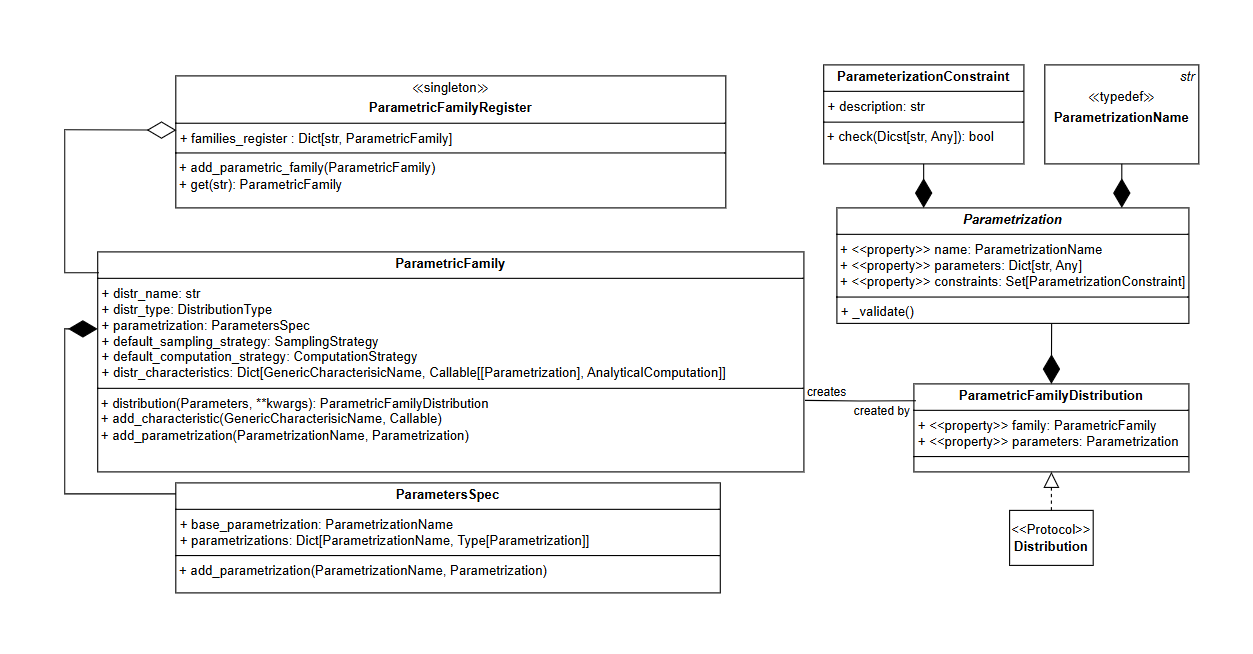
\includegraphics[width=\figurewidth]{assets/images/families-class-diagram.png}
    \caption{Диаграмма классов модуля families}
    \label{fig:class-diagram-families}
\end{figure}

Реестр семейств, используется, чтобы в будущем можно было реализовывать переходы между распределениями из семейств, при каких-то операциях

Каждое семейство является объектом класса \texttt{ParametricFamily}. Это позволяет использовать систему с реестром, а также:
\begin{itemizecmp}
    \item Добавлять пользовательские параметризации для распределений;
    \item Добавлять новые \texttt{AnalyticalComputation} для распределений,
\end{itemizecmp}
не модифицируя исходный код семейства. 

На данный момент за работу с несколькими параметризациями отвечает класс \texttt{ParametrizationSpec}. Его объекты описывают какие параметризации есть у семейства, и кто из них является канонической. Сейчас используется следующий механизм: все аналитические вычисления задаются в базовой параметризации, далее каждая параметризация указывает, как из нее получить базовую параметризацию. 

\subsubsection{Основные компоненты системы}

\noindent \texttt{ParametricFamiliesRegister} (Реестр параметрических семейств)
\begin{itemize}[noitemsep, topsep=0pt, parsep=0pt]
    \item \textbf{Назначение}: Синглтон-класс для глобальной регистрации и доступа ко всем параметрическим семействам.\item \textbf{Поля}:
    \begin{itemizecmp}
        \item \texttt{\_instance} - единственный экземпляр реестра
        \item \texttt{\_registered\_families} - словарь зарегистрированных семейств
    \end{itemizecmp}
    \item \textbf{Методы}:
    \begin{itemizecmp}
        \item \texttt{get(name)} - получение семейства по имени
        \item \texttt{register(family)} - регистрация нового семейства
    \end{itemizecmp}
\end{itemize}

\noindent \texttt{ParametrizationConstraint} (Ограничение параметризации)
\begin{itemize}[noitemsep, topsep=0pt, parsep=0pt]
    \item \textbf{Назначение}: Контейнер для ограничений на значения параметров распределения.

    \item \textbf{Поля}:
    \begin{itemizecmp}
        \item \texttt{description} - текстовое описание ограничения
        \item \texttt{check} - функция проверки ограничения
    \end{itemizecmp}
\end{itemize}

\noindent \texttt{Parametrization} (Абстрактный класс параметризации)
\begin{itemize}[noitemsep, topsep=0pt, parsep=0pt]
    \item \textbf{Назначение}: Абстрактный базовый класс для всех параметризаций распределений.

    \item \textbf{Поля}:
    \begin{itemizecmp}
        \item \texttt{constraints} - список ограничений параметров
    \end{itemizecmp}

    \item \textbf{Абстрактные свойства}:
    \begin{itemizecmp}
        \item \texttt{name} - имя параметризации
        \item \texttt{parameters} - словарь параметров
    \end{itemizecmp}

    \item \textbf{Методы}:
    \begin{itemizecmp}
        \item \texttt{validate()} - проверка всех ограничений
        \item \texttt{transform\_to\_base\_parametrization()} - преобразование к базовой параметризации.
    \end{itemizecmp}
\end{itemize}

\noindent \texttt{ParametrizationSpec} (Спецификация параметризаций)
    \begin{itemize}[noitemsep, topsep=0pt, parsep=0pt]
    \item \textbf{Назначение}: Контейнер для управления множественными параметризациями семейства.

    \item \textbf{Поля}:
    \begin{itemizecmp}
        \item \texttt{parametrizations} - словарь всех параметризаций
        \item \texttt{base\_parametrization\_name} - имя базовой параметризации
    \end{itemizecmp}

    \item \textbf{Методы}:
    \begin{itemizecmp}
        \item \texttt{base} - получение класса базовой параметризации
        \item \texttt{add\_parametrization()} - добавление новой параметризации
        \item \texttt{get\_base\_parameters()} - преобразование параметров к базовой форме
    \end{itemizecmp}
\end{itemize}


\noindent \texttt{ParametricFamily} (Параметрическое семейство)
\begin{itemize}[noitemsep, topsep=0pt, parsep=0pt]
    \item \textbf{Назначение}: Представление семейства распределений с различными параметризациями.

    \item \textbf{Поля}:
    \begin{itemizecmp}
        \item \texttt{name} - имя семейства
        \item \texttt{distr\_type} - тип распределения
        \item \texttt{parametrizations} - спецификация параметризаций
        \item \texttt{distr\_characteristics} - характеристики распределения
        \item \texttt{sampling\_strategy} - стратегия семплирования
        \item \texttt{computation\_strategy} - стратегия вычислений
    \end{itemizecmp}

    \item \textbf{Методы}:
    \begin{itemizecmp}
        \item \texttt{\_\_call\_\_()} - создание экземпляра распределения
    \end{itemizecmp}
\end{itemize}


\noindent \texttt{ParametricFamilyDistribution} (Конкретное распределение)
\begin{itemize}[noitemsep, topsep=0pt, parsep=0pt]
    \item \textbf{Назначение}: Конкретный экземпляр распределения с определенными параметрами. Реализует протокол \texttt{Distribution}

    \item \textbf{Поля}:
    \begin{itemizecmp}
        \item \texttt{distr\_name} - имя семейства
        \item \texttt{distribution\_type} - тип распределения
        \item \texttt{parameters} - параметры распределения
    \end{itemizecmp}

    \item \textbf{Свойства}:
    \begin{itemizecmp}
        \item \texttt{family} - ссылка на родительское семейство
    \end{itemizecmp}
\end{itemize}

\subsubsection{Типичные сценарии использования}

\paragraph{Определение нового семейства распределений}
Пользователь создает новое параметрическое семейство, определяя:
\begin{itemizecmp}
    \item Различные параметризации (каноническая, mean-var, etc.)
    \item Ограничения на параметры
    \item Функции для вычисления характеристик (PDF, CDF, etc.), доступные аналитически 
    \item Стратегии семплирования и вычислений
\end{itemizecmp}

\paragraph{Создание экземпляра распределения}
Пользователь создает конкретное распределение, указывая:
\begin{itemizecmp}
    \item Имя семейства
    \item Параметризацию (как минимум одну)
    \item Значения параметров
\end{itemizecmp}

\paragraph{Вычисление характеристик распределения}
Система автоматически:
\begin{itemizecmp}
    \item Проверяет корректность параметров
    \item При необходимости преобразует к базовой параметризации
    \item Вычисляет запрошенные характеристики
\end{itemizecmp}

\paragraph{Генерация выборок}
Используется зарегистрированная стратегия семплирования для генерации данных из распределения.


\end{document}